We pause here to reflect on the implication of our results
in \SEC\ref{sec:varmarg_opt} - \ref{sec:varapprox_opt}.  Namely, for
joint Gaussian variational $q(x,y)$ all optimality conditions are
satisfied by joint moment matching.  Thus, the same moment-matched
joint Gaussian is optimal for all three variational estimators.  For
the approximation $\Iml$, joint moment matching is equivalent to
optimizing an upper bound on error, but is not globally optimal in
general.  We conclude this section with additional properties of these
estimators.  For example, it is trivial to show that they obey the
following ordering:
%% The $\Imarg$ and $\Ipost$ are often useful because they are bounds. $\Iml$, on 
%% the other hand, is neither an upper bound or lower bound, however this 
%% approximation can be placed between the variational marginal and variational 
%% posterior bounds.\\
\begin{lemma}
  For any $q_m(x)$ and $q_p(x\mid y)$, $\Ipost\leq\Iml\leq\Imarg$.
  \label{lemma:MIOrder}
\end{lemma}
Thus, $\Iml$ is never the least accurate out of all three methods. If
$\Iml$ is an over approximation, it is a tighter upper bound than
$\Imarg$ and the converse holds if it is an under approximation (it is
a tighter than $\Ipost$). We can also ask when $\Iml$ is closer in
absolute error than either of the bounds
\begin{lemma}\label{lemma:AbsPostError}
  For a variational $q_m(x)$ and $q_p(x\mid y)$, if 
  \begin{enumerate}
    \item If $\KL{p(X\mid Y)}{q(X\mid Y)}\geq \frac{1}{2}\KL{p(X)}{q(X)}$ 
    then $\Iml$ has lower error than $\Ipost$
    \item If $\KL{p(X)}{q(X)}\geq \frac{1}{2}\KL{p(X\mid Y)}{q(X\mid Y)}$ 
    then $\Iml$ has lower error than $\Imarg$
  \end{enumerate}
\end{lemma}
While these conditions cannot be checked in practice they do offer
some insight.  For example, if $q_m(x)$ approximates $p(x)$ about as
well as $q_p(x\mid y)$ approximates $p(x\mid y)$ (in KL) then $\Iml$ is the
best approximation to use.

\paragraph{Moment matching stationary point} is not always a local minimum to the 
optimization of $\Iml$. Consider \FIG\ref{fig:MMoptimal} where a two
dimensional Gaussian is moment matched to Gaussian mixture models. All
of the parameters of the moment matched Gaussian are held constant but
the correlation parameter, $\rho$, is varied an the absolute error of
$\Iml$ is plotted. In one case, the minimum is found and any changed
value of $\rho$ results in a worse approximation of MI. However is the
second case, a local maximum is found, and we notice that there is a
range of values for $\rho$ that result in not only better
approximations of MI, but sometimes exact.  Exploring this property is
a topic of future work.

\begin{figure*}[!t]
  \centering
  \subfigure[Local minimum]{
    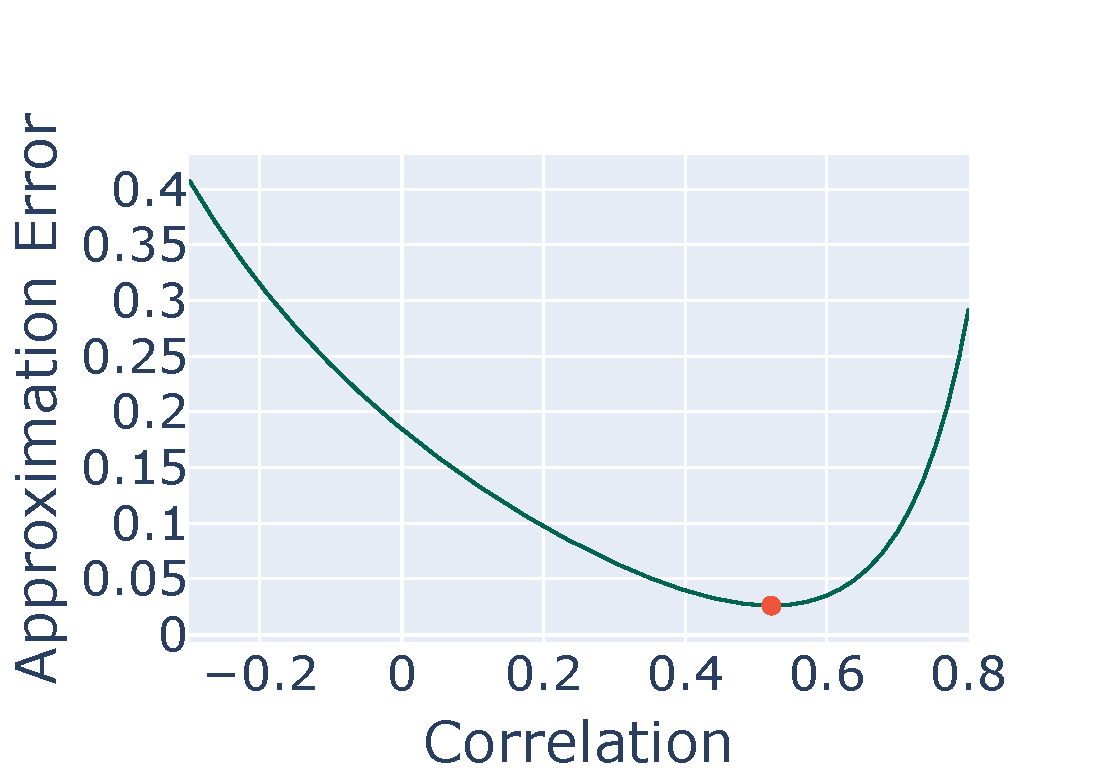
\includegraphics[width=.4\textwidth]{MMMinimum.pdf}
    }
  \subfigure[Local maximum]{
  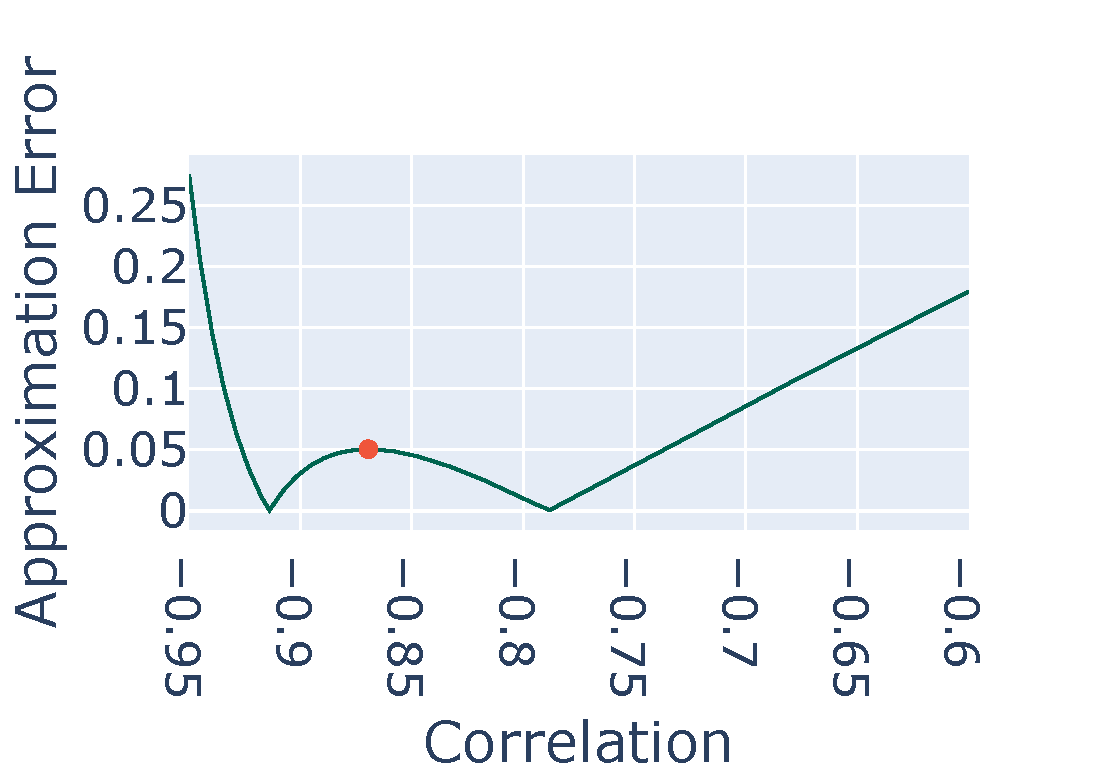
\includegraphics[width=.4\textwidth]{MMMaximum.pdf}
  }
  \caption{\small\textbf{Moment Matched Optimum} (a) The moment matching solution 
  (red) is the local minimum as a variational apprximation to a GMM. (b) For a 
  seperate GMM, the moment matched solution is a local maximum and there is a 
  range of values for $\rho$ that result in better approximation, and two that 
  result in exact values of MI.}
  \label{fig:MMoptimal}
\end{figure*}
